Este anexo apresenta os principais conceitos relacionados com a avaliação
da sustentabilidade segundo segundo os fines do projeto SustenAgro,
e como foram usados no processo de avaliação de sustentabilidade.

\section{Sustentabilidade}

Não existe um consenso sobre a definição de sustentabilidade, mas
uma definição orientadora para os fins do presente projeto é a seguinte:
\begin{quotation}
``O desenvolvimento sustentável prevê o atendimento das necessidades
do presente sem comprometer a capacidade das gerações futuras de suprir
suas próprias necessidades, \foreignlanguage{english}{Brundtland Commission}''
\citet{Burton:1987,brundtland1987our}
\end{quotation}
Este conceito foi ratificado pela Conferência das Nações Unidas sobre
o Meio Ambiente e Desenvolvimento, a Rio-92 \citet{ehlers1996agricultura}
a Rio+20 \citet{ONU2012}, após do relatório \foreignlanguage{english}{Brundtland}
a ênfase do conceito desloca-se da integridade ambiental para o elemento
humano, gerando um equilíbrio entre as dimensões econômica, social
e ambiental\citet{van2005indicadores}.

\citet{gliessman2001agroecologia} teoriza que não há como encontrar
a sustentabilidade e, portanto, o seu conceito mais representativo,
pois a mesma permanece sempre no futuro, dado o compromisso que os
sistemas têm de garantir as necessidades das gerações futuras. Assim,
a sustentabilidade é algo relativo ao tempo, ou seja, um sistema pode
ser mais ou menos sustentável que outro dependendo do tempo em que
for avaliado e do entendimento da sustentabilidade neste contexto.

A sustentabilidade esta vinculada a vários domínios de conhecimento,
um deles é a sustentabilidade em agricultura, que é de especial interesse
na segurança alimentar. Em 2050 a população mundial atingirá 9.1 bilhões
de pessoas FAO (2013), o qual imporá enormes desafios para garantir
a sustentabilidade em meio do aumento de alimentos, por isso são necessários
incentivos e políticas para garantir a sustentabilidade em agricultura,
a través da geração de estratégias que permitam conhecer o estado
dos sistemas produtivos e melhorar segundo as necessidades identificadas.

Segundo \citet{van2008integrated} os sistemas agrícolas evoluem continuamente
e são afetados por uma gama de forças globais e locais, os aspectos
que mais influenciam na sustentabilidade da agricultura são os tecnológicos
e políticos, permitindo identificar e melhorar diversos aspectos da
produção agrícola. 

Uma estrategia para quantificar a sustentabilidade são a definição
métodos e metodologias de avaliação, as quais utilizam indicadores,
um exemplo deste enfoque é exposto por \citet{AlkanOlsson:2009} que
desenvolveu um \foreignlanguage{english}{\emph{framework}} de indicadores
que relaciona de uma maneira consistente as dimensões ambiental, econômica
e social do desenvolvimento sustentável, seu principal benefício é
uma relativa simplicidade na apresentação da informação e a possibilidade
de vincular os indicadores com objetivos políticos de cada dimensão
da sustentabilidade e assim facilitar a comparação dos impactos das
novas políticas em cada dimensão.

\section{Dimensões da Sustentabilidade}

As dimensões da sustentabilidade são classificações que permitem identificar
e agrupar conceitos de sustentabilidade\citep{AlkanOlsson:2009}.,
dependendo da teoria de sustentabilidade escolhida, existem diversas
propostas de dimensões que podem ser usadas segundo a finalidade da
pesquisa, um exemplo desta classificação é a assumida na pesquisa
de \citet{oliveira:2013} onde são definidas seis dimensões da sustentabilidade:
Ambiental, Social, Agrícola/Industrial, Produtos/Subprodutos, Tecnológica
e Política.

No caso do sistema SustenAgro determinou-se pela equipe de especialistas
em sustentabilidade fazer uma divisão segundo a proposta do Relatório
Brundtland \citep{brundtland1987our}, onde foram identificadas as
três dimensões da sustentabilidade: ambiental, social e econômica,
as quais têm a mesma importância gerando um equilíbrio.

Ditas dimensões são sistemas complexos que integram fenômenos de natureza
diversa \citep{simon1991architecture}, integrando três subsistemas:
(i) o subsistema ambiental que fornece as condições físicas, químicas
e biológicas que suportam o desenvolvimento das culturas, (ii) o subsistema
social que integra organizações e pessoas que realizam a produção,
relacionando-se internamente e externamente com os sistemas produtivos
e (iii) o subsistema econômico que estabelece as condiciones de oferta
e demanda dos produtos e subprodutos do sistema de produção agrícola;
das interações entre estes subsistemas, emerge um comportamento complexo
que requer uma abordagem holística e inter-relacionada para suportar
a tomada de decisões que garantam a sustentabilidade do sistema em
analise.

A Figura \ref{fig:sustainability_spheres} representa as três dimensões
com a sustentabilidade como a interseção entre elas.

\begin{figure}[h]
\begin{centering}
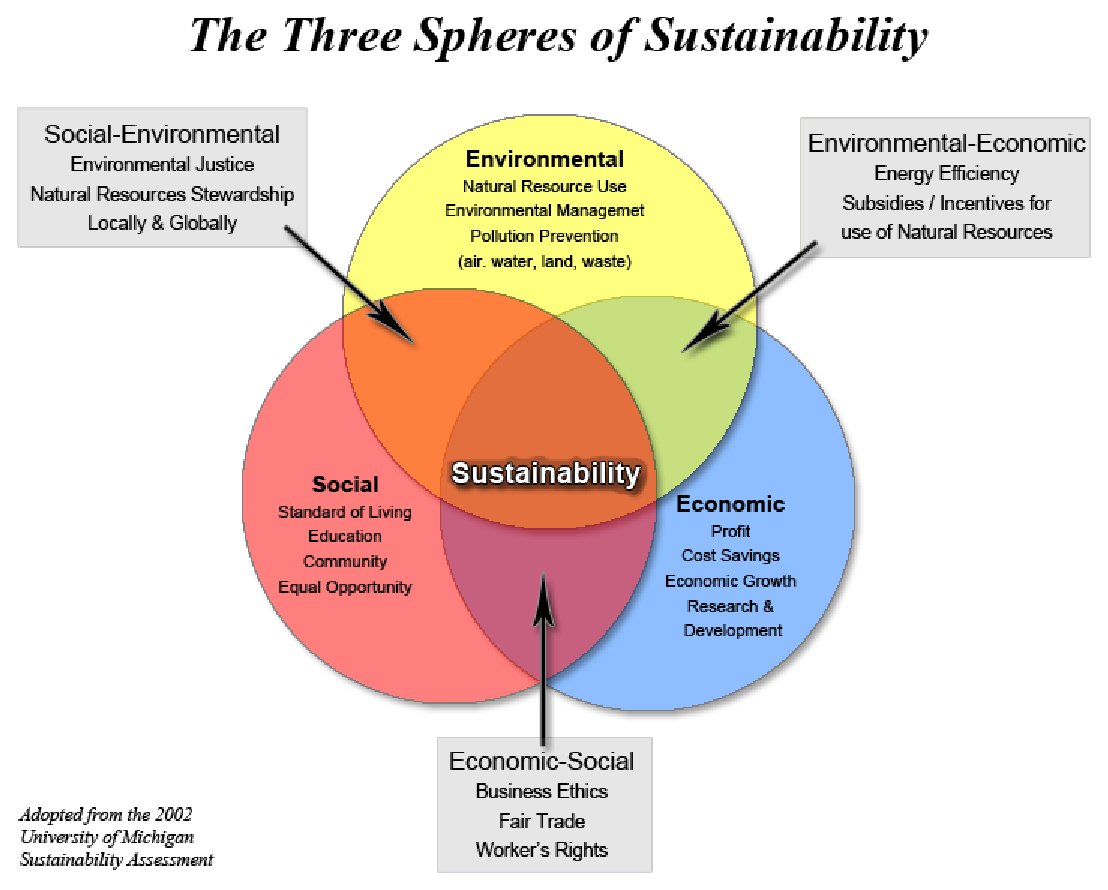
\includegraphics[width=1\columnwidth]{figures/sustainability_spheres}
\par\end{centering}
\caption{Dimensões da sustentabilidade \label{fig:sustainability_spheres}}
\end{figure}

\footnote{Tomada de: http://www.vanderbilt.edu/sustainvu/cms/files/sustainability\_spheres.png}Essas
dimensões serão usadas como contendedores gerais dos conceitos de
sustentabilidade em agricultura permitindo agrupar conceitos relacionados.

\section{Critérios de sustentabilidade}

São variáveis transversais quantitativas e qualitativas, que são monitoradas
regularmente para determinar os efeitos das atividades de intervenção
ou não-intervenção do sistema em avaliação \citet{deusdara2001criterios},
que estabelecem os preceitos de orientação para que os indicadores
sejam representativos para a sustentabilidade.

Cada indicador deverá atender pelo menos um dos critérios de sustentabilidade
para ser considerado um bom indicador de sustentabilidade, os critérios
de sustentabilidade escolhidos pela equipe de especialistas são:
\begin{itemize}
\item Produtividade: Relacionado a eficiência e custos.
\item Estabilidade: Capacidade do ecossistema de absorver perturbações e
permanecer inalterado (CEPAL\nomenclature{CEPAL}{Economic Commission for Latin America and the Caribbean}/PNUMA\nomenclature{PNUMA}{Programa das Nações Unidas para o Meio Ambiente},
1994) \citet{moura2002indicadores}
\item Equidade: Distribuição dos produtos do agroecossistema entre produtores
e consumidores (Dias Junior, 2000) \citet{moura2002indicadores}
\item Resiliência: Capacidade do ecossistema de retornar ao estado original
após de uma perturbação (CEPAL/PNUMA, 1994) \citep{moura2002indicadores}
\item Autonomia: Grau de integração entre as partes constituintes do agroecossistema
e o ambiente externo no fluxo de materiais, energia e informação (Fernández,
1995) \citep{moura2002indicadores}Autonomia: Grau de integração do
agroecossistema no fluxo de materiais, energia e informação entre
as partes constituintes e entre o agroecossistema e o ambiente externo
(Fernández, 1995) \citep{moura2002indicadores}
\end{itemize}
Esses critérios guiam o desenvolvimento dos conceitos mais relevantes
das metodologias de avaliação de sustentabilidade, os indicadores,
e assim determinar instrumentos de medição que representem os aspectos
críticos do sistema em termos de sustentabilidade.

\section{Atributos Norteadores}

Embora a orientação para a elaboração de todas as variáveis relacionadas
a projetos de sustentabilidade devam atender pelo menos a três pilares:
ambiental, econômico, social, os atributos norteadores são formulados
para garantir as diretrizes no levantamento e validação dos indicadores,
e assim ter um modelo da sustentabilidade dos sistemas de produção
agrícola.

Após a agregação dos dados será possível visualizar as informações
disponíveis e eventuais lacunas para a sistematização dos componentes
dos sistemas produtivos em termos dos requisitos de sustentabilidade.
Em uma primeira instância, devem ser levantados dados referentes ao
solo, clima, água, ar, produção agroindustrial, divisas geradas, mão
de obra envolvida, empregos gerados, doações/benefícios indiretos
à sociedade, biodiversidade, etc.

Uma proposta dos atributos norteadores é a seguinte:
\begin{itemize}
\item Dimensão Ambiental: solo, hídrico, clima, entre outros
\item Dimensão Social: saúde, capacitação, emprego, renda, entre outros
\item Dimensão Econômica: industrial, agrícola, produtividade, custo, entre
outros
\end{itemize}
Os atributos norteadores foram aplicados nos modelos do sistema SustenAgro
como contentores de indicadores os quais classificaram e relacionam
os indicadores em subgrupos das três dimensões da sustentabilidade,
permitindo desta maneira a organização e agrupamento do conhecimento
do domínio.

\section{Metodo SustenAgro}

Devido à importância da sustentabilidade, especialmente nos sistemas
de produção agrícola, foram desenvolvidas varias métodos para avaliar
o estado desses sistemas, existindo varias tendências segundo o tipo
de sistema produtivo e o contexto deles.

A Embrapa Meio Ambiente coordenou e financiou o projeto SustenAgro
com a finalidade de definir um método de avaliação da sustentabilidade
no sistema produtivo de cana-de-açúcar no centro sul do Brasil, as
características dele são descritas nas figuras \ref{fig:SustenAgro_Description}
e \ref{fig:SustenAgro_Details}, no qual foram originados os indicadores
de sustentabilidade e o método de avaliação \citep{oliveira:2013,BRUMATTI:2015}.

\vfill{}

\pagebreak{}

\begin{figure}[H]
\begin{centering}
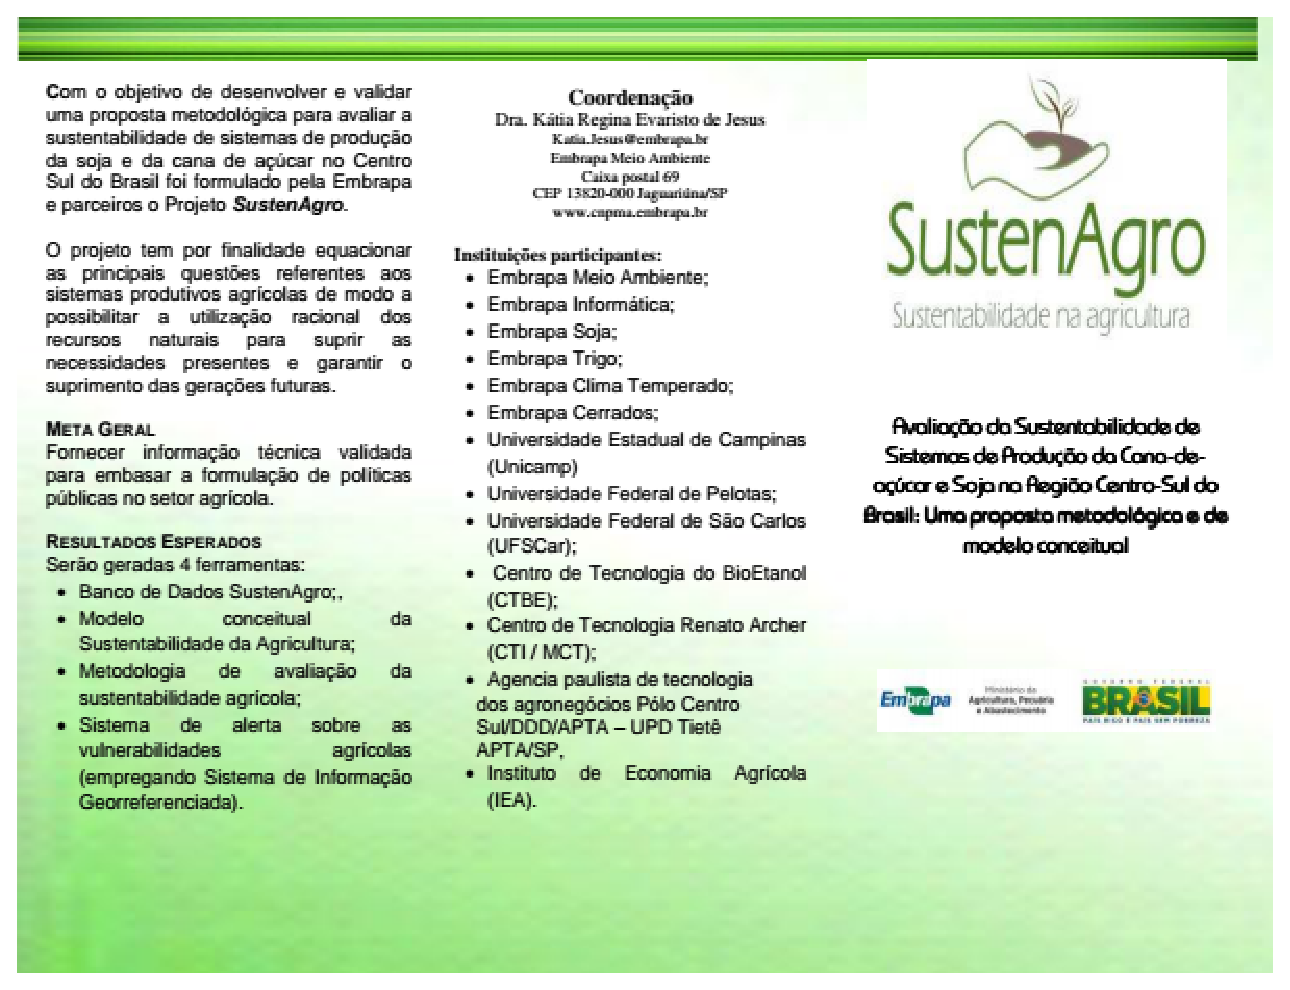
\includegraphics[width=1\columnwidth]{figures/folderEmbrapa1}
\par\end{centering}
\caption{Descrição geral do projeto SustenAgro \label{fig:SustenAgro_Description}}
\end{figure}

\begin{figure}[H]
\begin{centering}
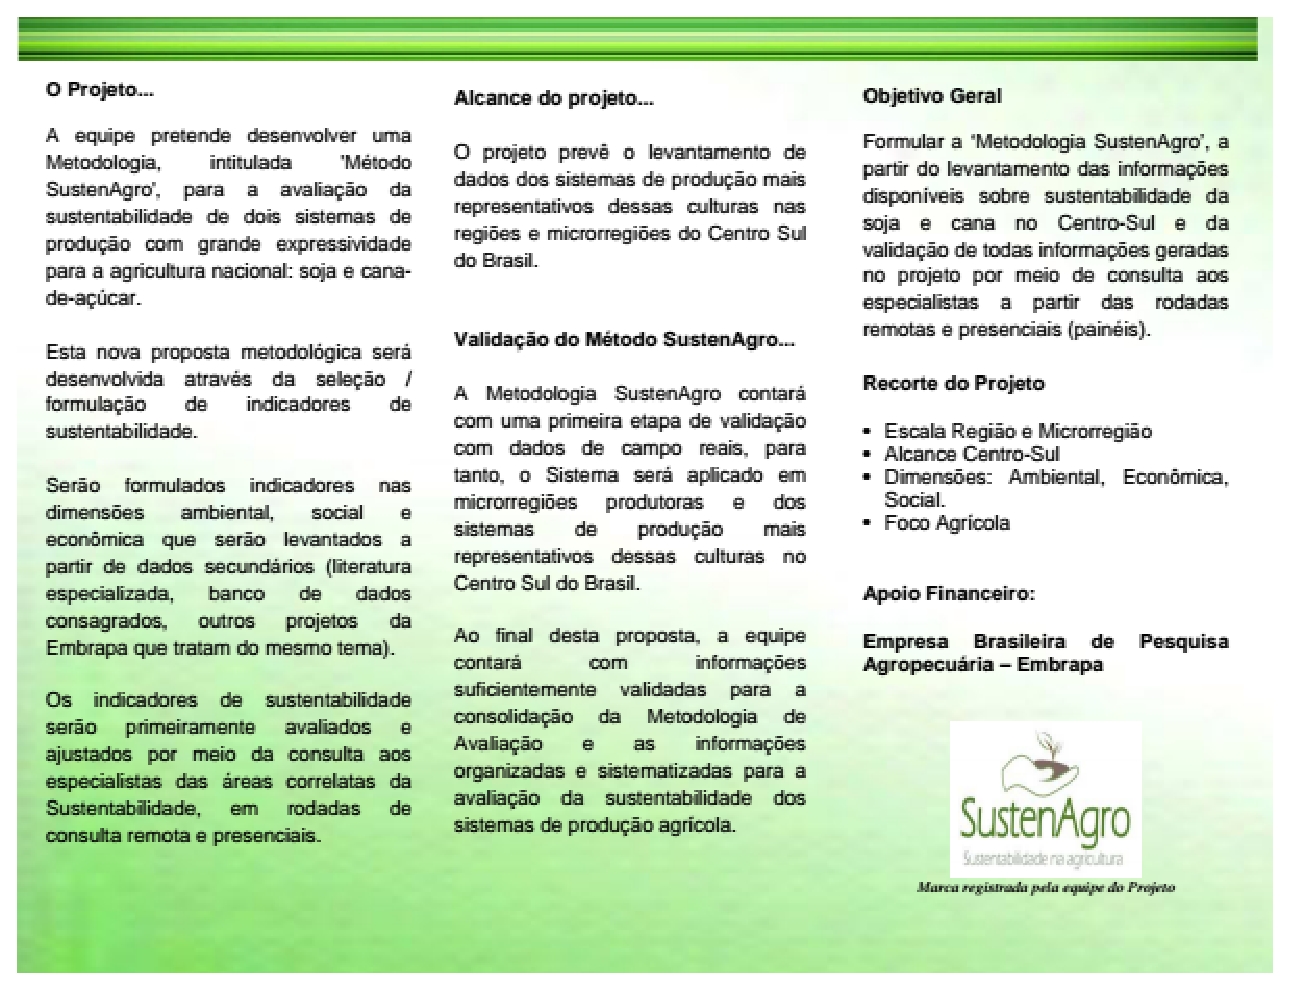
\includegraphics[width=1\columnwidth]{figures/folderEmbrapa2}
\par\end{centering}
\caption{Descrição especifica do projeto SustenAgro \label{fig:SustenAgro_Details}}
\end{figure}

O método SustenAgro foi construído a partir de literatura cientifica
e de instituições de pesquisa como (IBGE\footnote{IBGE: Brazilian Institute of Geography and Statistics, http://www.ibge.gov.br/home/},
CONAB \footnote{CONAB: National Supply Company, http://www.conab.gov.br/})
e validados por meio da técnica Delphi de consultas aos especialistas.

O método esta composto de dos índices da eficiência e índice da sustentabilidade,
o índice da eficiência esta composto por dois fatores de eficiência
tecnológica no campo e na industria e o índice da sustentabilidade
está composto pelas dimensões ambientais, econômica e social.

\subsection*{Índice de eficiência:}

As equações para calcular o índice da eficiência são:

Formula de eficiência tecnologia no campo:

$efficiency(field)=\sum(CharacteristicsInTheField*RelevanceForTheProductionEnvironment)*correctionFactor(0.8)$

Formula de eficiência tecnologia na industria:

$efficiency(industry)=\sum(CharacteristicsOfProcessing*SugarcaneProcessingOptimization)*correctionFactor(0.2)$

Formula de eficiência produtiva e de costo:

$efficiencyAndCost=\sum(SugarcanEquality+\sum(Logistic+MarketVariables+Policies+Productivity))$

Índice de eficiência:

$EfficiencyIndex=\sum(efficiency(filed)+efficiency(industry))*efficiencyAndCost$

\subsection*{Índice de sustentabilidade}

As equações para calcular o índice de sustentabilidade são:

Formula de eficiência tecnologia no campo:

$EnvironmentalIndex=\sum(EnvironmentalIndicator*EnvironmentIndicatorWeight)$

Formula de eficiência tecnologia na industria:

$EconomicIndex=\sum(EconomicIndicator*EconomicIndicatorWeight)$

Formula de eficiência produtiva e de costo:

$SocialIndex=\sum(SocialIndicator*SocialIndicatorWeight)$

Índice de eficiência:

$SustainabilityIndex=\sum(EnvironmentalIndex+EconomicIndex+SocialIndex)/3$

\section{Matriz de sustentabilidade}

Os índices de eficiência e de sustentabilidade quantificam a sustentabilidade
de uma unidade produtiva, e são representados por meio de uma matriz
que tem como finalidade relacionar o resultado da avaliação com determinadas
classificações correspondentes a cada uns dos quadrantes da matriz,
a figura \ref{fig:Matriz-de-sustentabilidade} representa cada uma
das classificações com os limiares correspondentes a cada índice.

\begin{figure}[h]
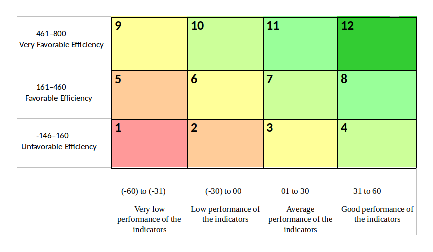
\includegraphics[width=0.8\columnwidth]{figures/SustaiabilityMatrixDesign}

\caption{Matriz de sustentabilidade \label{fig:Matriz-de-sustentabilidade}}

\end{figure}


\section{Conclusões}

O método de avaliação de sustentabilidade foi validado pelos especialistas
e depois de varias iterações definiu-se uma versão estável, que foi
usada no desenvolvimento do Sistema SustenAgro, dito método é mantido
e atualizado pela Embrapa Meio Ambiente e os desenvolvedores de software
garantem que ele se aplique corretamente mas não tem responsabilidade
nenhuma pelas consequências do uso dele.
